% Unofficial University of Cambridge Poster Template
% https://github.com/andiac/gemini-cam
% a fork of https://github.com/anishathalye/gemini
% also refer to https://github.com/k4rtik/uchicago-poster

\documentclass[final]{beamer}

% ====================
% Packages
% ====================

\usepackage[T1]{fontenc}
\usepackage{lmodern}
\usepackage[size=custom,width=91.44,height=60.96,scale=0.9]{beamerposter}
\usetheme{gemini}
\usecolortheme{uchicago}
% 36x24in is narrower than the template default, so the title column is tighter.
% One step down from the theme default (\Huge) keeps the title on two lines.
\setbeamerfont{headline title}{size=\huge,series=\bfseries}
\usepackage{graphicx}
\usepackage{booktabs}
\usepackage[numbers]{natbib}
\usepackage{tikz}
\usepackage{pgfplots}
\pgfplotsset{compat=1.14}
\usepackage{anyfontsize}

% ====================
% Lengths
% ====================

% If you have N columns, choose \sepwidth and \colwidth such that
% (N+1)*\sepwidth + N*\colwidth = \paperwidth
\newlength{\sepwidth}
\newlength{\colwidth}
\setlength{\sepwidth}{0.025\paperwidth}
\setlength{\colwidth}{0.3\paperwidth}

\newcommand{\separatorcolumn}{\begin{column}{\sepwidth}\end{column}}

% ====================
% Title
% ====================

% Line break is manual: beamerposter does not wrap the title automatically.
% The short title in [] is what goes into the PDF metadata -- without it,
% hyperref hits the \\ while building the metadata string and errors out.
\title[Graph Neural Network Modeling of Breast MRI Vascular Networks for Treatment Response Prediction]{Graph Neural Network Modeling of Breast MRI Vascular \\ Networks for Treatment Response Prediction}

\author{Spencer Venancio \inst{1} \and Sarit Bose \inst{2} \and Aakrithi Ram \inst{3}\and Advisor: Anna Woodard, PhD \inst{4}}

% The student affiliations share a line; the hosting institute gets its own so it
% does not read as a fourth school in a run-on list. \samelineand is \qquad, so
% only \\ actually breaks the line.
\institute[shortinst]{%
 \inst{1} University of Wisconsin--Madison \samelineand
 \inst{2} Neuqua Valley High School \samelineand
 \inst{3} Bergen County Academies \\[0.5ex]
 \inst{4} Data Science Institute, University of Chicago}

% ====================
% Footer (optional)
% ====================

% TODO: fill in before printing. Left as visible TODOs rather than the upstream
% example.com/"ABC Conference" placeholders, which look real enough to survive
% to the printer by accident.
\footercontent{
 github.com/dsi-clinic/vanguard \hfill
  University of Chicago Data Science Institute Summer Research Symposium \hfill
  svenancio@wisc.edu}
% (this whole block can be deleted to remove the footer)

% ====================
% Logo (optional)
% ====================

% Three logos: two on the left, one on the right.
%
% Provenance -- all official, all with real alpha:
%   uchicago_logo_white.png  University-Logo.zip, PNG_RGB_Digital/Reverse
%                            University Logo_1Color_White_RGB.png -- the
%                            shield+wordmark lockup, which UChicago's guidelines
%                            prefer over the seal for general communications.
%                            https://creative.uchicago.edu/logos-and-identity-elements
%   dsi_logo_white.pdf       https://datascience.uchicago.edu/wp-content/uploads/
%                            2023/01/DSI_Logo_Color@1x.svg, converted with
%                            `rsvg-convert -f pdf` so it stays vector at print size.
%                            The name is misleading: that file is entirely #FFFFFF
%                            (the knockout the DSI site uses on its dark footer).
%                            The actual colour version is DSI_Logo_Color-2@1x.svg.
%
% These are the knockout ("Reverse ... White") variants, meant for dark
% backgrounds -- which is what the maroon headline needs. Do not swap in a
% colour DSI logo without also lightening the headline: its maroon ink is
% RGB(139,0,33) against a RGB(128,0,0) bar, so it disappears.
%
% Two constraints worth keeping if you swap these:
%   - The theme reserves \maxlogowidth on BOTH sides of the title, taking the
%     wider of the two sides. A wide logo block on one side eats into the title
%     twice over, squeezing it towards one word per line.
%   - Do not use .eps. An EPS logo makes lualatex exit nonzero even though the
%     PDF comes out fine, which then wedges latexmk. PNG and PDF are both fine.
\logoleft{%
  \begin{tabular}{@{}l@{}}
    
\includegraphics[height=5.5cm]{logos/uchicago_logo_white.png} \\[1.5ex]
    
\includegraphics[height=4.6cm]{logos/dsi_logo_white.pdf}
  \end{tabular}%
}
% Right side carries the author institutions, left the host. The two school marks
% sit in a row under UW so the block stays about as wide as it is tall -- see the
% \maxlogowidth note above.
%
% Provenance (both official school sources, both with real alpha):
%   nvhs_wildcat.png  https://resources.finalsite.net/images/v1745596249/ipsdorg/
%                     pwceoev9pdbw5f653ytp/nvhs.png -- the Neuqua Valley mark on
%                     Indian Prairie District 204's own Finalsite CDN. Only
%                     325x200, so ~145 DPI at the height set below; it is the
%                     largest the district publishes. Navy-and-gold with a white
%                     outer stroke, which is what keeps it legible on maroon.
%   bca_seal.png      https://bca-admissions.bergen.org/images/logo.png -- the
%                     Bergen County Academies seal from their admissions site,
%                     866x866.
% Rejected: bergen.org's BergenN.png is the *district* mark (Bergen County
% Special Services Technical Schools), not BCA.
% Heights are deliberately unequal: UW-Madison is the first author's institution
% and leads, with the two schools set smaller beneath it as contributor credits.
\logoright{%
  \begin{tabular}{@{}c@{}}
    
\includegraphics[height=6.2cm]{logos/uw_madison_white.pdf} \\[1.6ex]
    
\includegraphics[height=2.8cm]{logos/nvhs_wildcat.png}\hspace{2em}%
    
\includegraphics[height=2.8cm]{logos/bca_seal.png}
  \end{tabular}%
}

% ====================
% Body
% ====================

\begin{document}

% Note: the upstream template placed its logo here as an absolutely-positioned
% tikzpicture overlay, which sits on top of the headline instead of inside it --
% so a title of any length runs straight through the logo. That is why the logos
% are set with the theme's own \logoleft/\logoright hooks in the preamble
% instead: those reserve space and keep the title clear of them.

\begin{frame}[t]
\begin{columns}[t]
\separatorcolumn

\begin{column}{\colwidth}

  \begin{block}{Introduction + Motivation}

    Breast cancer is the most common cancer in women worldwide, and neoadjuvant
    chemotherapy (NAC) is widely given before surgery. Only about a third of
    patients achieve a \textbf{pathologic complete response (pCR)} to NAC, which is
    associated with improved survival outcomes. NAC is an intensive treatment that
    can have significant side effects, and patients who do not achieve pCR may
    require additional treatment. We would like to develop methods to predict
    which patients will respond to NAC, so that we can better tailor treatment
    plans and improve outcomes.
     
  \end{block}

  \begin{block}{Ultrafast MRI Dataset}

    The dataset consists of \textbf{ultrafast breast MRI} from a single institution:
    181 labeled exams across 143 patients, of which 179 are analyzed here. Each
    exam is a dynamic contrast-enhanced series with precontrast baseline frames and
    pCR labels; 35\% of exams are pCR-positive. Exams come from three sub-sources
    (\texttt{simbiosys}, \texttt{uch\_nac}, \texttt{her2\_naclike}) whose
    acquisition timing differs materially --- 13--24 frames over 96--480\,s.

  \end{block}

  \begin{alertblock}{Graph Representation}

    \begin{figure}
      \centering
      
\includegraphics[width=0.75 \linewidth]{figures/graph_representation.pdf}
      \caption{Vascular segments and junctions are converted into graph nodes
      and edges.}
    \end{figure}

    We represent the vascular network of each patient's tumor as a graph, and 
    propose 3 different methods of constructing the graph from the MRI scans.
    In the following let $\mathcal{G} = (\mathcal{V}, \mathcal{E})$ be a graph.

    \begin{itemize}
      \item  \textbf{Voxel-as-node} Let the set of nodes $\mathcal{V}_{\text{vox}}$ be the set 
      of all voxels, and let the set of edges $\mathcal{E}_{\text{vox}}$
      be the set of all pairs of adjacent voxels. In this representation, each 
      voxel is a node, and edges connect adjacent voxels.

       \item \textbf{Junction-as-node} Let $\mathcal{V}_{\text{jun}}$ be the 
       set of all junctions (i.e. $e \in \mathcal{E}_{\text{vox}}$ with $\mathrm{deg}(e) > 2$) 
       in the vascular network, and let $\mathcal{E}_{\text{jun}}$ be the set
       of all pairs of junctions that are connected by a vascular segment.

       \item \textbf{Segement-as-node} Let $\mathcal{V}_{\text{seg}}$ be the 
       set of all vascular segments, and let $\mathcal{E}_{\text{seg}}$ be the 
       set of all pairs of segments that are connected at their endpoints. In this 
       representation, each segment is a node, and edges connect adjacent segments.
     
    \end{itemize}
  \end{alertblock}

\end{column}

\separatorcolumn

\begin{column}{\colwidth}

  % Pipeline and architecture are one block: the two used to end and begin with
  % the same sentence ("a GNN is trained to predict treatment response from the
  % graph representation"), and each figure carries most of its own explanation.
  % Merging them frees a block header and about eighty words for the pretext-task
  % section below.
  \begin{block}{Prediction Pipeline and GNN Architecture}

    \begin{figure}
      \centering
      
\includegraphics[width=\linewidth]{figures/dsi-pipeline.pdf}
      \caption{End-to-end prediction pipeline.}
    \end{figure}

    Vessel segmentation is performed using a \textbf{nnU-Net model}, which labels
    each voxel as vessel or background. The segmentation is simplified into a
    one-voxel wide network of vessels using the \textbf{tc4d} algorithm, then
    converted into a graph using one of the three representations above.

    A \textbf{graph neural network (GNN)} predicts treatment response from that
    graph. Successive \textbf{graph convolution (GCN)} layers aggregate information
    from neighboring nodes, a global pooling layer collapses all nodes into a
    fixed-size representation of the entire graph, and a fully connected layer maps
    that representation to a binary prediction (pCR vs. non-pCR).

    % Vector PDF (25.3 x 9.1 cm, no raster layers), so it scales cleanly. Figure
    % text scales with the include width, not the poster size: at 0.4\textwidth
    % these labels rendered at roughly 40% of the size drawn.
    \begin{figure}
      \centering
      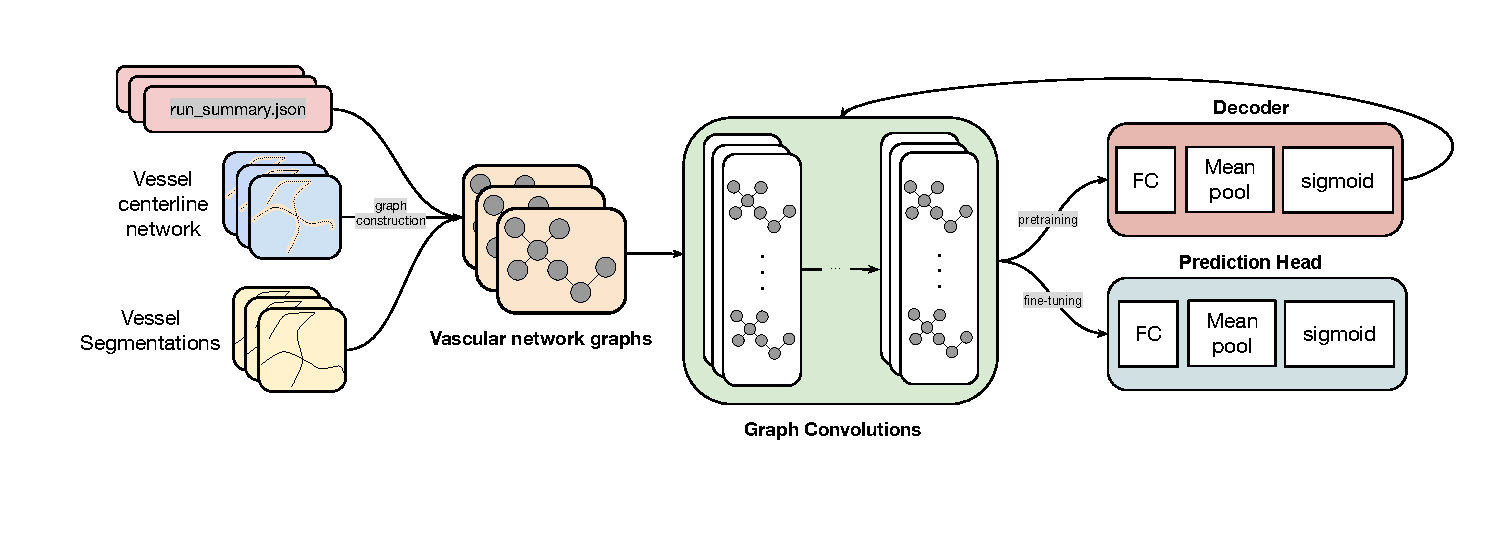
\includegraphics[width=\linewidth]{figures/GNN_arch.pdf}
      \caption{GNN architecture: 4D DCE-MRI through the vessel graph to a pCR
      probability.}
    \end{figure}

  \end{block}

  \begin{block}{Self-supervised Pretraining}

    To improve the performance of the GNN, we use a \textbf{self-supervised pretraining}
    approach. The GNN is first trained to predict \emph{per node} the future contrast
    enhancement, where it learns to predict contrast flow through the network.

    Each contrast curve is cut into non-overlapping windows. Shown the frames on an
    input horizon $[t_1, t_L]$, the model predicts every node's enhancement over the
    following horizon $(t_L, t_{L+H}]$, scored by mean absolute error against the
    measured signal. Predictions are conditioned on \textbf{elapsed seconds}
    $\tau = t - t_1$ rather than on frame index, so the irregular ultrafast cadence
    is handled directly.

  \end{block}

\end{column}

\separatorcolumn

\begin{column}{\colwidth}

  \begin{exampleblock}{Results}

    % Regenerate with figures/make_results_figure.py when new results land.
    % Preliminary: these numbers are expected to move before final submission.
    \begin{figure}
      \centering
      
\includegraphics[width=\linewidth]{figures/results_auc.pdf}
      \caption{Pooled out-of-fold AUC, bootstrap 95\% CI, shared folds.
      \emph{Preliminary.}}
    \end{figure}

    Every arm carrying the full enhancement-kinetic feature set clusters between
    \textbf{0.607 and 0.624} AUC. The paired difference between the best GNN and
    the best tabular baseline is consistent with zero, $+0.002$ $[-0.041, 0.046]$.

    A GNN restricted to two features (peak time and radius) sits at chance,
    $0.492$, placing the signal in the enhancement kinetics rather than in the
    graph. So far feature content moves the metric; model class and graph
    representation do not.

    \heading{Protocol confound}

    Acquisition timing differs by sub-source, and four of the seven kinetic
    features depend on it. A protocol-only model with no imaging scores $0.593$;
    regressing protocol out per fold leaves $0.539$ --- read the vessel signal as
    the bracket $[0.539, 0.613]$.

  \end{exampleblock}

  \begin{block}{Reproducibility}
    All code is publicly available on GitHub: vessel segmentation, graph
    construction, GNN training and evaluation, plus instructions to reproduce
    these results.
  \end{block}

  \begin{block}{Conclusion}

    We built an end-to-end pipeline that turns ultrafast breast MRI into a vessel
    graph and predicts pCR with a GNN. The vasculature carries some signal, but no
    graph representation yet beats a tabular summary of the same node features, and
    part of the pooled signal tracks acquisition protocol rather than physiology.
    Quantifying what survives protocol adjustment, and whether pretraining helps,
    are the next steps.

   
  \end{block}

  \begin{block}{References}

    \nocite{*}
    \footnotesize{\bibliographystyle{plainnat}\bibliography{poster}}

  \end{block}

\end{column}

\separatorcolumn
\end{columns}
\end{frame}

\end{document}
